\begin{PROBLEM}
	\p
	دنباله‌ای با دامنه‌ی نامحدود از اشکال زیر وجود دارد. این سه شکل، به ترتیب از چپ به راست، سه عضو اول این دنباله هستند.‌
	 $a_i$
	را معادل تعداد پاره‌خط‌های موجود در عضو 
	$i$-ام این دنباله در نظر بگیرید.
	جمله‌ی عمومی دنباله $a_i$ را بر حسب
	$n$
	به‌دست آورید.
    \begin{center}
     	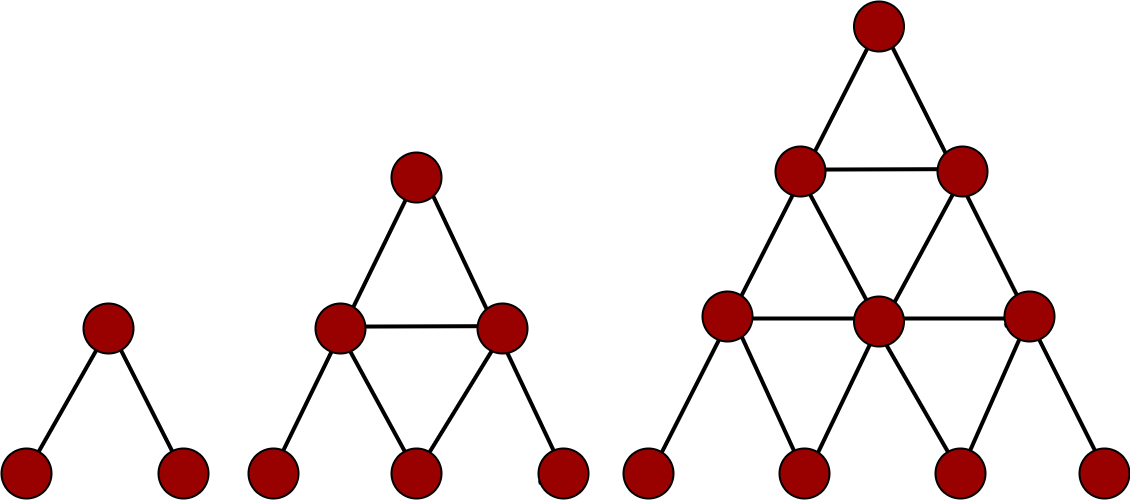
\includegraphics[scale=0.2]{./2.png}
    \end{center}
    \SOLUTION{
    \p
       	$$a_1 = 2$$
       	$$a_2 = a_1 + (1\times 2 + 1)$$
        $$a_3 = a_2 + (3\times 2 + 2)$$
		$$\vdots$$
		$$a_n = a_{n-1} + (n\times 2 + (n-1))$$
		\begin{center}
				$\rule{0.4\textwidth}{0.8pt}$
				\Huge{+}
		\end{center}
		$$a_n = a_1 + 2(2 + 3 + 4 +\cdots+ n) + 1 + 2 + \cdots + (n-1)$$
		$$a_1 + 2(\frac{n(n + 1)}{2} - 1) + \frac{(n - 1)n}{2}$$
		$$a_1 = 2 \rightarrow a_n = n((n + 1) + \frac{n -1}{2})$$
		$$a_n = \frac{n(3n + 1)}{2}$$
        }
\end{PROBLEM}